\section{Introduction}

With the advent of Internet of Things, the evolution of mobile computing, and the emergence of real-time applications, the processing of an exponentially increasing volume of data must be performed in a timely fashion, i.e., with minimum latency. Despite the elasticity and vast computing power of existing cloud platforms, the access to these resources involves multiple hops of network communication, adding prohibitive latency to requests' processing. Such limitation has the following implications:

\begin{enumerate}

\item Cloud services may fail to satisfy the requirements of real-time and low-latency client applications; and

\item Offloading of delay-sensitive computation from devices with constrained resources to cloud servers is unlikely to work due to network-latency.

\end{enumerate}

%\subsection{Edge Computing}

To reduce network latency, data processing must be performed closer to where it is produced and consumed. In accordance with this principle, the emerging paradigm of edge computing~\cite{} states that computing power should be pushed from centralized datacenters to the edge of the network. The realization of this paradigm, however, still poses many challenges:

%
--- First, a highly distributed edge infrastructure is not expected to exhibit virtually unlimited resources as cloud datacenters. This limitation requires a more efficient allocation of edge resources. Current models based on virtualization and containerization, although successfully adopted by cloud providers, may not be feasible in the context of edge computing.

--- Second, cloud services cover very large areas in which requests from clients are always expected. In contrast, edge infrastructure features a fine-grained coverage area~\cite{Dehos14millimeter5g} where edge services would remain idle whenever clients are absent in their coverage area. Therefore, to optimize the usage of edge resources, edge infrastructure should support the opportunistic deployment of services.

%, accessible through well-known Internet names, edge services 

--- Third, different types of edge computing infrastructure may exist, including servers located at cellular base stations, temporarily placed nearby public events, and inside buildings and houses to provide support for smart environment applications. The eventual co-existence of edge alternatives would require the client-side participation on the decision of which alternative to use.

--- Last but not least, considering the high availability and elasticity of cloud computing and the opportunistic nature of edge computing, the later should complement rather than replace the former. This vision also extends to the computation that may opportunistically be offloaded from resource constrained mobile devices to nearby edge servers. In this sense, cloud, edge, and mobile computing should be seen as a \textit{computational continuum}, as depicted in Figure~\ref{fig:continuum-overall}.

\begin{figure}[tbp]
	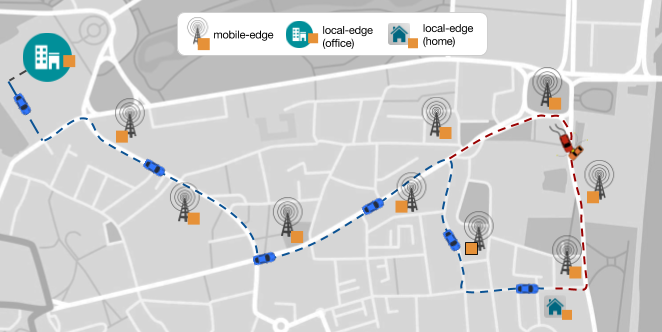
\includegraphics[width=0.8\textwidth]{figs/continuum.png}
	\caption{Computational Continuum formed by Mobile/IoT devices, Edge Datacenters and Cloud}
	\label{fig:continuum}
\end{figure}

 

%--- Last but not least, cloud servers should not be disregarded as a part of the Cloud-to-Edge continuum. %not sure whether to call it Cloud-to-Things or Cloud-to-Edge
%First, because client applications may still rely on Cloud backends for traditional, non delay-sensitive computation. Second, because edge servers may be unavailable from the certain locations. Thus, client applications must rely on a runtime mechanism to discover and negotiate the use of nearby edge infrastructure. As the alternative infrastructures (including the cloud) may exhibit uneven loads in different moments, the decision of which to use, must take into account their current status as well as the client application requirements in terms of latency and computational power. 


%Finally, to avoid increasing the burden of application development, computation to be executed at the edge should follow, to the extent possible, a common architecture and implementation with respect to its cloud counterpart. The same applies to the computation that may be offloaded from resource constrained devices to nearby edge infrastructure.  

%\subsection{Serverless Computing}

%Serverless computing~\cite{Roberts:2016, Hendrickson:2016}, also known as Functions-as-a-Service (FaaS)~\cite{MateosFaaster17}, emerged as an alternative execution model within cloud computing. In particular, its name derives from the fact that server management and capacity planning decisions are hidden from the software application engineers. Instead, third party providers of the serverless platform dynamically manage resource allocation and sharing for the execution of different types of computational tasks, known as \textit{functions}. Nowadays, all major cloud vendors provide serverless runtimes an associated ecosystem of services. 
%
%Among its main advantages, the serverless model is cost- and resource-efficient in comparison to virtual machine and container-based provisioning models, which generally involve significant periods of underutilization or idle time. In previous work~\cite{GarrigaMendonca2017}, we discussed the suitability of a serverless architecture to enable low-latency applications to use edge computing computational resources in an efficient, scalable and automated way. In this work, serverless computing is further explored in the realization of the computational continuum composed also by cloud and mobile devices by means of a unified model.

%mobile devices could make use of compute runtimes deployed at nearby edge servers to extend their capabilities. Notwithstanding the potential of such combination, a complete model for its realization is still missing~\cite{NasticServerlessEdge17}. 

\subsection{Contributions of this Work}

In this paper, we propose A3-E --- \textit{(A)wareness, (A)cquisition, (A)llocation and (E)ngagement} --- a unified model that empowers applications to leverage the computation continuum formed by cloud, edge, and mobile computing. In accordance with our previous work~\cite{GarrigaMendonca2017}, A3-E is based on the serverless computing paradigm~\cite{Hendrickson:2016,baldini2017serverless}. In specific, A3-E explores the function-as-a-service (FaaS) model~\cite{MateosFaaster17} to allow stateless functions to be quickly deployed and exposed as services, providing an efficient and scalable allocation of computing resources. A3-E further extends FaaS with the complete automation of services life-cycle, including the acquisition and installation of service artifacts by servers. Such an autonomy releases developers and administrators from the burden of deployment and maintenance and further supports the materialization of a fine-grained distribution of the network edge and the computational continuum as a whole. %Contribution: Scalable Edge Computing


As demonstrated through different experiments, client applications can rely on services dynamically selected and implemented as functions that are executable locally, in the edge, or in the cloud. Such a selection is performed according to the application requirements and the actual context of the continuum as perceived by the client. The experiments have shown a XX\% reduction of latency when edge services were used instead of cloud services, and a YY\% decrease of battery consumption when computation was offloaded from the mobile device to nearby edge server. Finally, experiments with an augmented reality application have also shown the feasibility of A3-E model in the realization of the computational continuum, with a single client application been able to seamlessly alternate local, edge, and cloud according to its requirements and monitored context.


%Last but not least, our contribution also includes a reference architecture for the realization of the proposed model. 

%\subsection{Paper Organization}

The rest of this paper is organized as follows. Section~\ref{sec:motivation} describes the main motivation behind this work, including application scenarios and the computational continuum. Section~\ref{sec:background} provides a brief background on the main topics and concepts used by this work. Section~\ref{sec:proposal} provides a detailed description of the A3-E model, whereas Section~\ref{sec:implementation} details both the client-side implementation for Android platform and the server-side implementation for edge-computing. Section~\ref{sec:evaluation} reports on the experiments performed to evaluate our proposal with an augment reality application. Section~\ref{sec:related} presents related work. Finally, Section~\ref{sec:conclusions} concludes the paper and delineates future work.




